\subsection{Performance Analysis of Algorithms}
\label{subsec:data process}

We now evaluate our proposed
algorithms with the experimental setup described in
Sections~\ref{subsec:ichannel} and \ref{subsec:insitu}.
The metrics of
{\it Accuracy} and {\it Throughput Gap} are used in the evaluation.
We consider each second of the in-field trace and
observe the frequency band that had the highest 
throughput.  The \emph{Accuracy} is defined as the percentage of 
best band predictions that match the observed optimal band, where a prediction
is made each second.  Conversely, the \emph{Throughput Gap} is defined
as the difference between the throughput observed on the optimal band
and the throughput achieved by the predicted best band over the
throughput of the observed optimal band. 
In the situation where the optimal band is not chosen, the throughput could be close between the chosen and optimal bands, meaning that the
incorrect band choice did not result in a large throughput loss. Thus, the 
\emph{Throughput Gap} metric captures the severity of the incorrect choice.

%\begin{align}
%\label{equation:df accuracy}
%Accuracy = \frac{Correct\ Prediction\ Slots}{All\ Predict\ Time\ Slots}
%\end{align}
%
%\emph{Throughput Gap} is the deference between the performance of estimation throughput and measured best throughput as defined in Formula \ref{equation:df gap}.
%
%\begin{align}
%\label{equation:df gap}
%Throughput\ Gap = \frac{\sum{Max\ Tpt- Estimate\ Band\ Tpt}}{\sum{Max\ Tpt}}
%\end{align}

Since the \emph{SNR-based Throughput Look-up Algorithm} requires only 
emulator-based training, the \emph{Accuracy} and \emph{Throughput Gap} can 
be calculated for all loops of the in-field trace.  However, the 
\emph{Location-based Look-up Algorithm} and \emph{Region-based Decision
Tree Algorithm} require in-field training. Thus, the data set must be
divided into a training set and testing set for evaluation.

\begin{figure}
%\vspace{-0.0in}
\centering
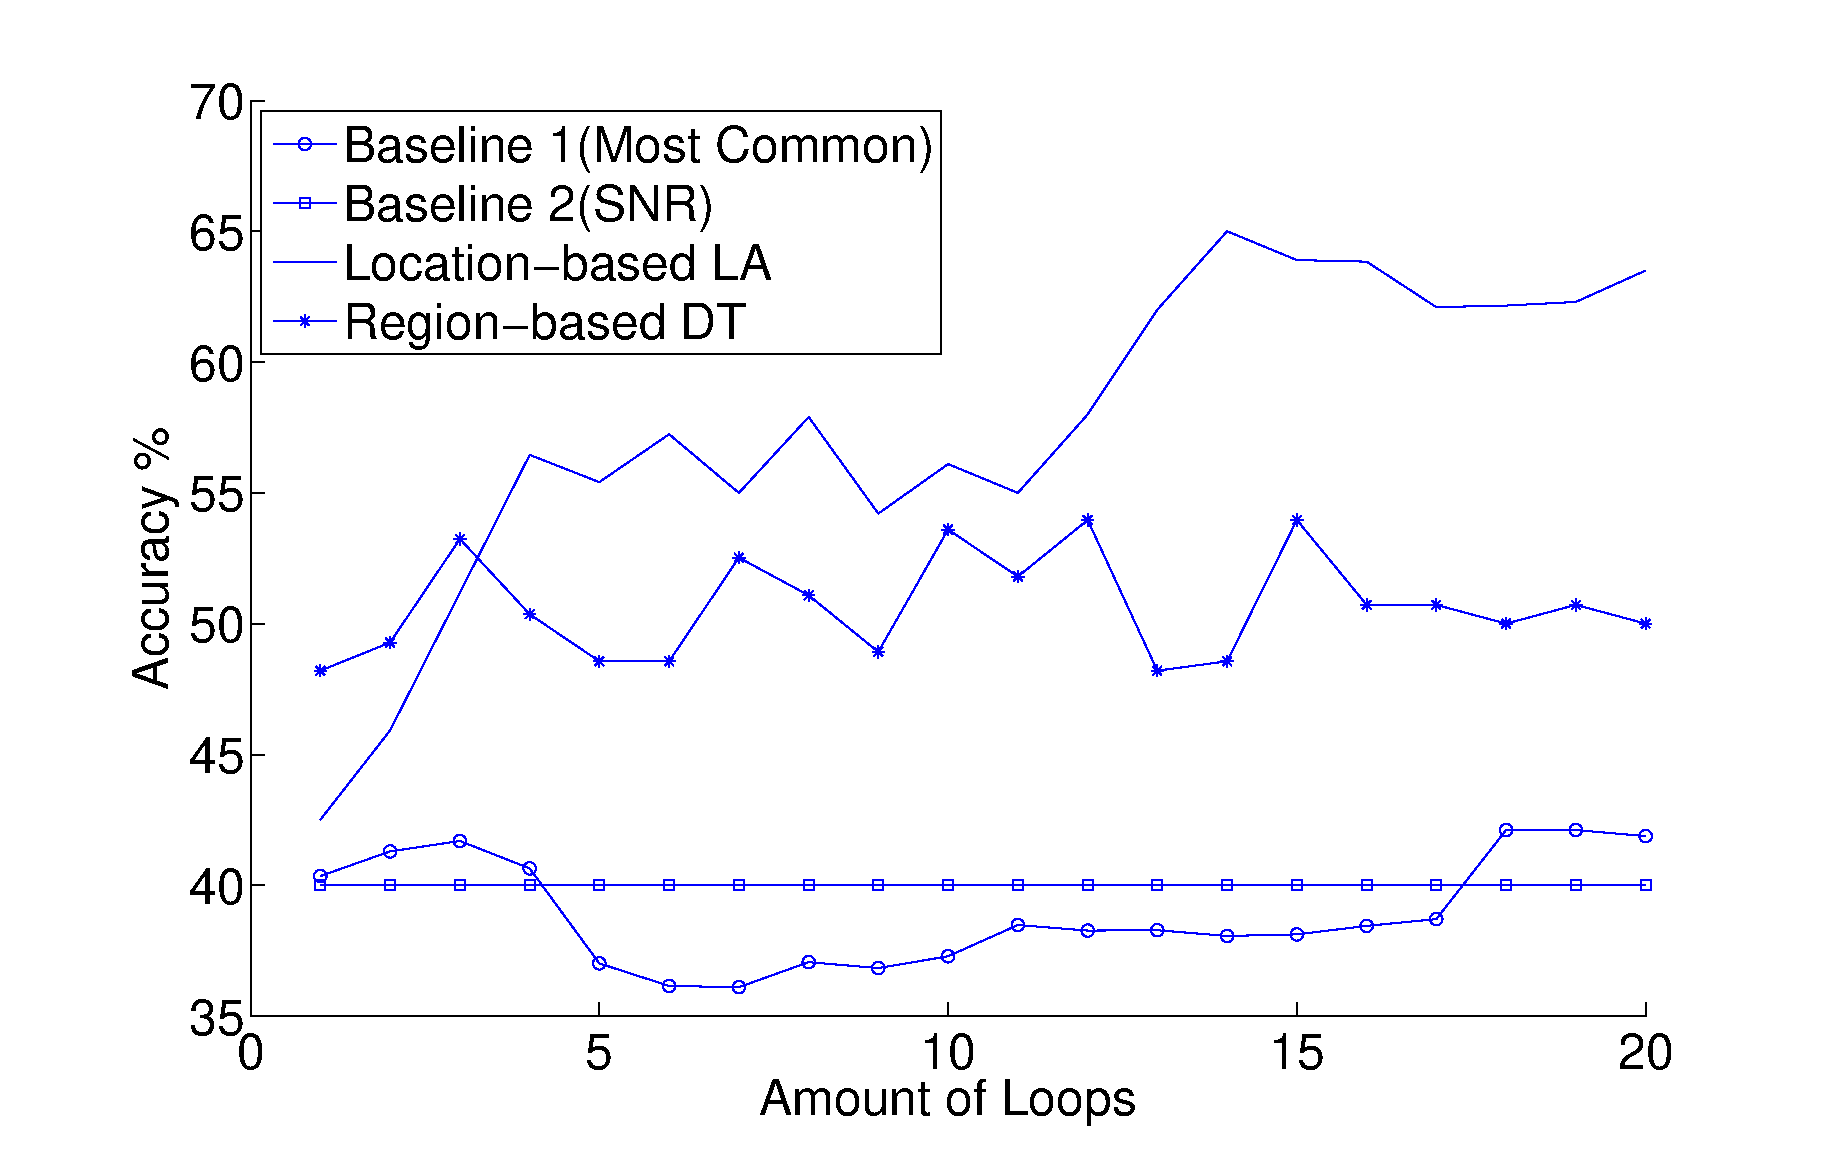
\includegraphics[width=68mm]{figures/performance_accuracy}
\vspace{-0.1in}
\caption{Accuracy of the four multiband algorithms.}
\label{fig:performance}
%\vspace{-0.0in}
\end{figure}

In Figure \ref{fig:performance}, we show the aforementioned \emph{Accuracy}
of the four multiband algorithms in selecting the band with the highest
throughput. The x-axis represents the number of loops around the
block of the mobile transmitter (shown in 
Figure~\ref{fig:infield}) that will be used by the machine-learning-based
algorithms. We use the same training and testing set to compare 
the \emph{Location-based Look-up Algorithm} and \emph{Region-based
Decision Tree Algorithm}. From the results, we observe the following:

\begin{itemize}
\item
At each loop, the first baseline algorithm, \emph{Most Commonly-Selected
Band}, uses the band with the greatest long-term average of the percentage
of time that band yields the highest throughput over the previous loops.
The accuracy ranges from 36.1\% to 42.9\%.
\item
The second baseline algorithm, \emph{SNR-based Throughput Look-up},
maintains 39.2\% across all the loops since it relies only on 
emulator-based training.
\item 
The \emph{Region-based Decision Tree Algorithm} has an accuracy ranging
from 48.2\% to 54.0\% but contains many dips due to the relationship
between the context information and the distribution of the best band
choice changing on a loop-by-loop basis. Additional training data 
slightly improves the decision structure overall but primarily induces
additional noise in the training process.
\item 
The \emph{Location-based Look-up Algorithm} begins with an accuracy of
42.5\% but improves the most out of any algorithm to finish with an 
accuracy 62.5\% with the highest accuracy of 65.0\% occurring after loop 14.
Additional in-field training loops are likely to further improve the multiband
selection accuracy.
\end{itemize}

\begin{figure}
\vspace{-0.1in}
\centering
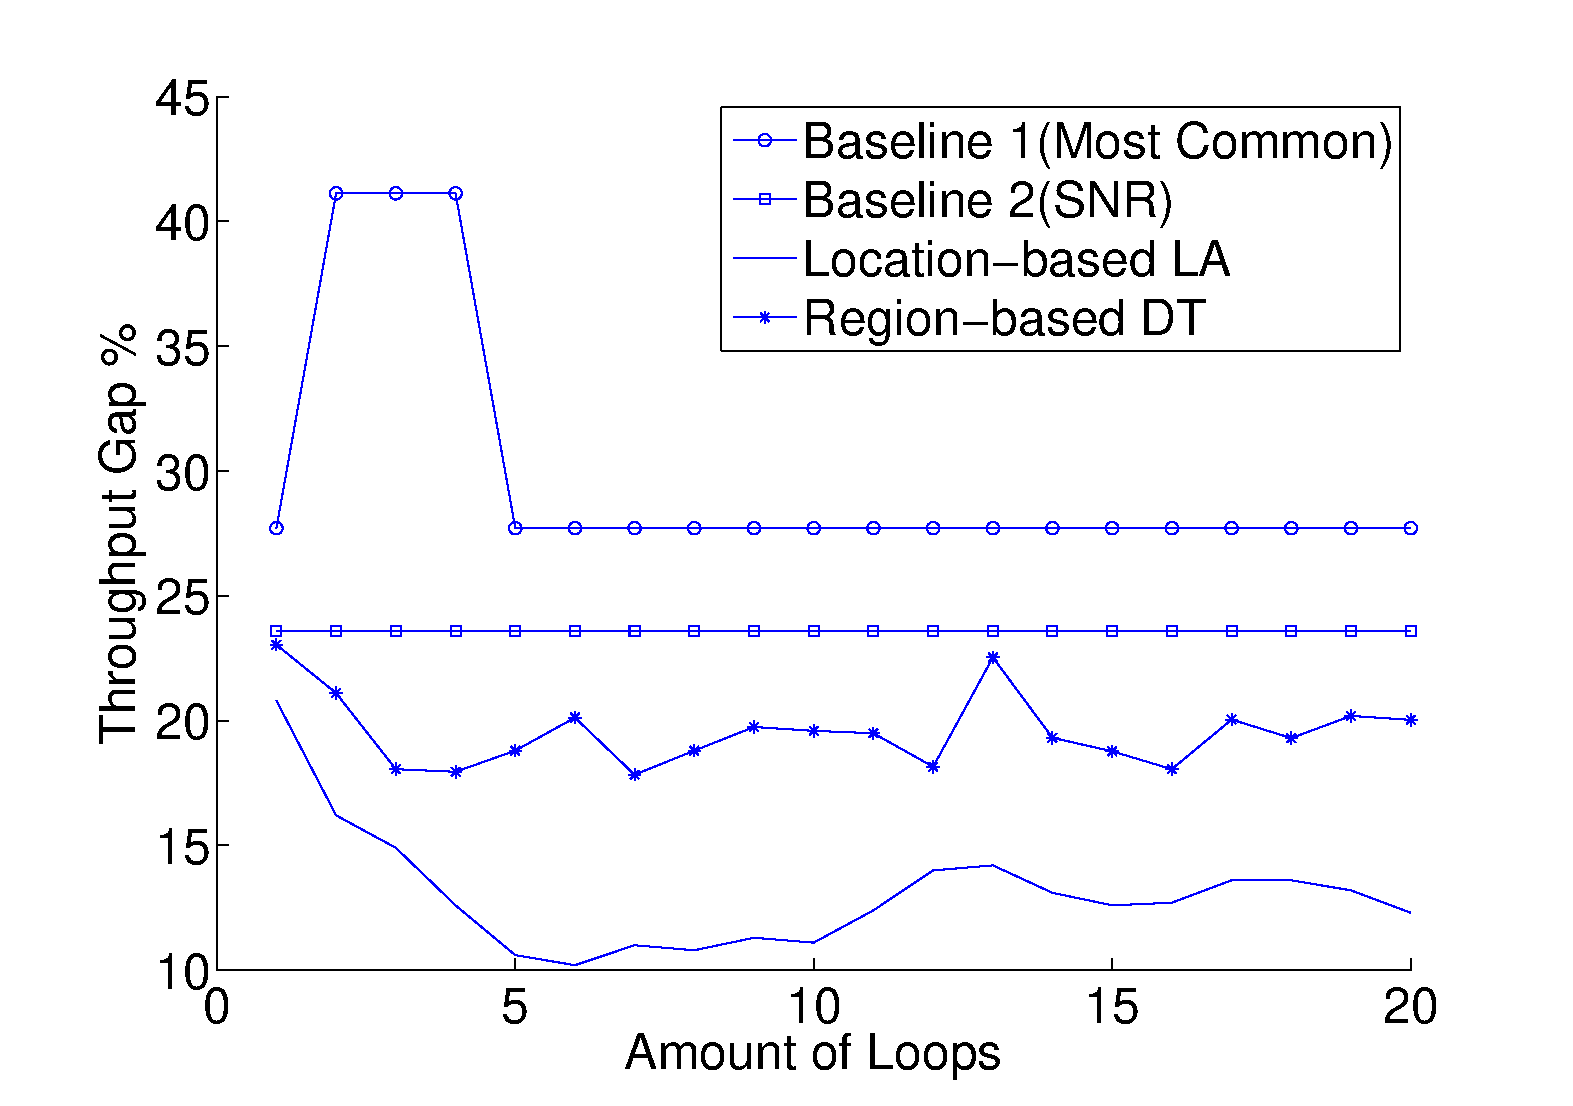
\includegraphics[width=65mm]{figures/performance_gap}
\vspace{-0.1in}
\caption{Throughput Gap of the four multiband algorithms.}
\label{fig:performance_gap}
\vspace{0.1in}
\end{figure}

Figure~\ref{fig:performance_gap}, 
depicts the \emph{Throughput Gap} of the four algorithms we evaluated and shows the following.

\begin{itemize}
\item
The \emph{Most Commonly-Selected Band Algorithm} has two different modes
of throughput gap based upon which band has the highest long-term 
percentage.  For loops 2-4, the choice is 5.8 GHz, which has a gap of 
41.1\% using the test set. For all other loops, the choice is 2.4 GHz, 
which has a gap of 27.7\%. 
\item 
The \emph{SNR-based Throughput Look-up Algorithm} shows a baseline  
performance of 23.6\% for the throughput gap.
\item 
The \emph{Region-based Decision Tree Algorithm} benefits from
additional training, going from a throughput gap of 23.0\% to 20.0\%.
Spatial and temporal changes to context information bring dips
to the curve as discussed earlier.
\item
Finally, the \emph{Location-based Look-up Algorithm} takes only 6 loops
of training to reach its lowest value of 10.2\% in terms of throughput
gap. From loops 1 to 20, the throughput gap goes from 20.8\% to 12.3\%,
which might still be improved upon with additional training.
\end{itemize}

\begin{figure}
%\vspace{-0.0in}
\centering
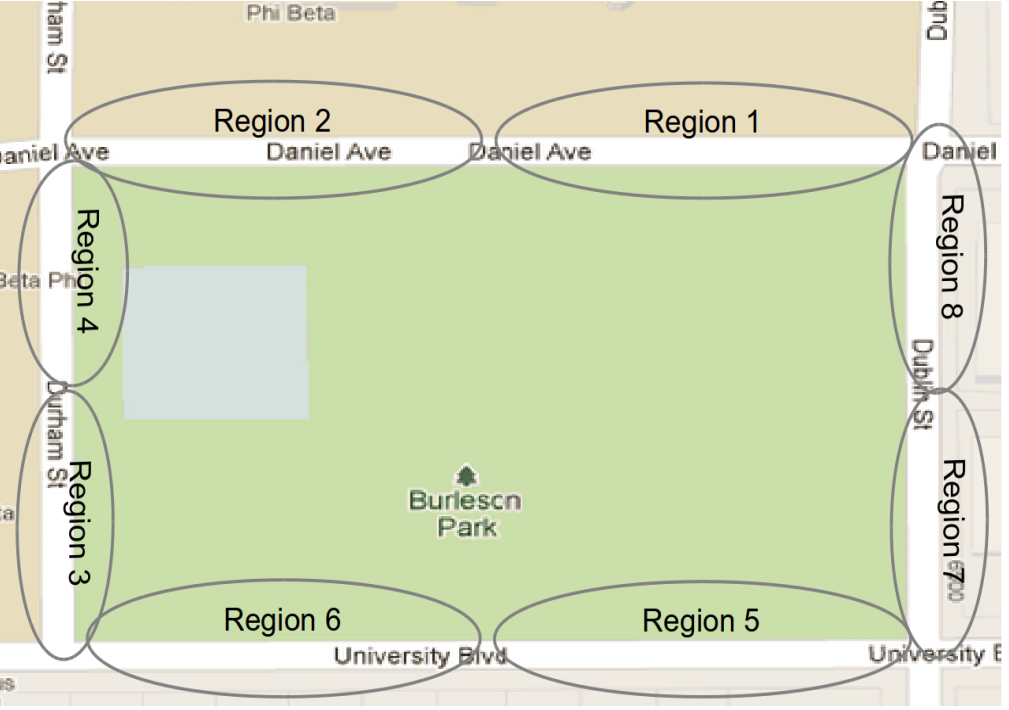
\includegraphics[width=75mm]{figures/region_map}
\vspace{-0.1in}
\caption{Spatially splitting experimental area into 8 regions.}
\label{fig:region map}
%\vspace{-0.0in}
\end{figure}

\begin{figure}
\vspace{-0.1in}
\centering
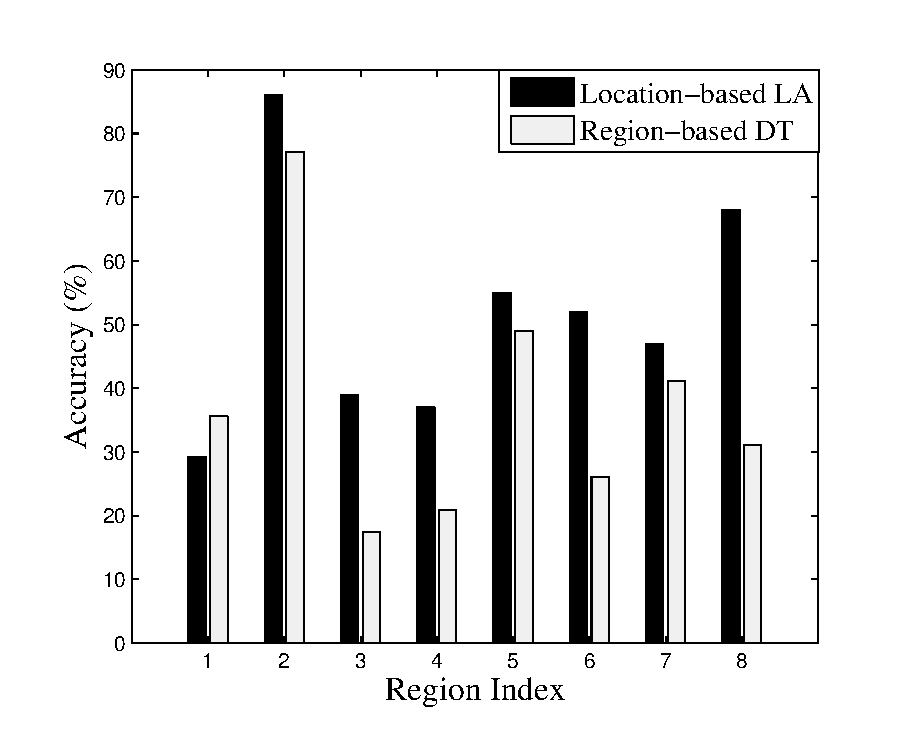
\includegraphics[width=65mm]{figures/mvsl}
\vspace{-0.1in}
\caption{Accuracy when dividing training set into 8 regions.}
\label{fig:mvsl}
\vspace{0.1in}
\end{figure}

We now consider the effect of further sub-dividing in-field experimental testing data into regions for our \emph{Location-based Look-up Algorithm} 
and \emph{Region-Based Decision Tree Algorithm}. To do so, we divide the    
loop around the park into eight regions as shown in Figure \ref{fig:region map},
which has two competing effects: (i.) Smaller regions allow similar experimental
data to be used in the training process, potentially improving the decision
structure. (ii.) For a given training set, dividing it into regions reduces
the number of training points for the machine learning algorithms, potentially
weakening the decision structure.  In Figure~\ref{fig:mvsl}, we observe 
the \emph{Accuracy} of the eight regions for both algorithms.
\begin{itemize}
\item
In all but Region 1, the \emph{Location-based Look-up Algorithm} has better 
performance than \emph{Region-based Decision Tree Algorithm}. The improved
accuracy of the former algorithm can be attributed to its ability to
distinguish each point's relative distance to the middle of the region
For the \emph{Region-based Decision Tree Algorithm}
to capture such a notion, the regions would have to be further sub-divided,
increasing the number of trees and reducing the training set per tree.
\item
For this training set, the reduction in training data caused by the
regional divisions had a net loss on the performance of the \emph{Region-based Decision Tree Algorithm}. However, if the training set was much larger
for a given area, the net effect of regional divisions could be positive.
\end{itemize}

%We have investigated the performance of the algorithms in one experimental data set and shown the gains of them. Multiband channels are complex system that knowing more information can make better decisions. 



